\documentclass[../main.tex]{subfiles}
%\graphicspath{{\subfix{images/}}}

\begin{document}
\label{sec:cyclotomic}

Cyclotomic polynomials are frequently used in the construction of homomorphic encryption schemes that are based on the ring learning with error (RLWE) problem \index{ring LWE} as we will see later in this tutorial. The motivations of using cyclotomic polynomials are the fact that cyclotomic fields have additional algebraic properties to reduce encryption scheme's time complexity and also make security proofs feasible by following the LWE proof paradigm. 
In this section, we will introduce the cyclotomic polynomials and the Galois groups of cyclotomic extensions.\index{cyclotomic extension} 
We have tried to make this section as self-contained as possible.
The appendix contains a more general treatment of field extensions and the Galois groups of field extensions for interested readers.
Useful references for material covered in this section include \cite{mukherjee2016cyclotomic}, \cite{conradcyclotomic} and \cite{porter15cyclotomic}. 


\subsection{Cyclotomic polynomials}
Cyclotomic polynomials\index{cyclotomic polynomial} are polynomials whose roots are the primitive roots of unity. To understand what it means, we define next. 

\begin{definition}
For any positive integer $n$, the $n$-th roots of unity\reversemarginpar\marginnote{\textit{Roots of unity}}\index{roots of unity} are the (complex) solutions to the equation $x^n = 1$, and there are $n$ solutions to the equation. 
% 
% A number $r$ is an \textbf{nth root of unity} for a positive integer $n$ if it satisfies $r^n=1$.
\end{definition}

\begin{theorem}\label{thm:roots of unity}
Let $n$ be a positive integer and define $\zeta_n = e^{2\pi i/n}$.
Then the set of all $n$-th roots of unity is given by 
\begin{equation}
    \{ \zeta_n^k \,|\, k = 0,1,\ldots, n-1 \},
\end{equation}
\end{theorem}
\begin{proof}
By Euler's formula\index{Euler's formula}, we have
\[ e^{2\pi i} = \cos(2\pi) + i \sin(2\pi) = 1 \]
and that $(e^{2\pi i})^k = e^{2k\pi i} = 1$ for all $k \in \{0,1,\ldots, n-1\}$.
To solve for $x^n = 1$, note that
\[ x^n = 1 = e^0 = e^{2\pi i} = e^{4\pi i} = e^{6\pi i} = \cdots = e^{2k\pi i}. \]
Raising each term to the power of $1/n$ yields
\[ x = (x^n)^{1/n} = 1 = e^{2\pi i/n} = e^{4\pi i/n} = e^{6\pi i/n} = \cdots = e^{2k\pi i/n}. \]
Therefore, there are $n$ distinct solutions to $x^n = 1$, each given by $\zeta_n^k$, for $k=0,1,\ldots,n-1$
\end{proof}

\iffalse
In the complex field $\C$, for example, both $\pm 1$ are the 2nd roots of unity. In general, the root $r$ can either be a real or complex number. So we can re-write the root $r$ as a complex number in the polar form as 
\begin{align*}
    r^n = 1 &= \cos 2\pi + i \sin 2\pi \\
    &= \cos 2k\pi + i \sin 2k\pi \\
    &= e^{2k \pi i}
\end{align*}
for $k \in [0, \infty)$. Hence, the nth root of unity in this representation is 
\begin{align*}
    r &= \cos 2k\pi/n + i \sin 2k\pi/n \\
    &= e^{2k\pi i/n} 
\end{align*}
for $k \in [0, n-1]$. The nth roots of unity is often denoted by the set $\{\zeta_n^0, \zeta_n^1, \dots, \zeta_n^{n-1}\}$, where $\zeta_n^0=1$ is always a root of itself. The subscript can be dropped if the context is clear. 
\fi

\begin{example}
The 1st root of unity is 1. The 2nd roots of unity are $\zeta_2^0=1$ and $\zeta_2^1=-1$. The 3rd roots of unity are $\zeta_3^0=1$, $\zeta_3^1=-\frac{1}{2}+i\frac{\sqrt{3}}{2}$ and $\zeta_3^2=-\frac{1}{2}-i\frac{\sqrt{3}}{2}$.
\end{example}

Geometrically, we can interpret the nth roots of unity as the points that are evenly spread on the unit circle in the complex plane, starting from 1 on the real axis. (The word ``cyclotomic'' means ''circle-dividing''.) Equivalently, they are the vertices of a regular n-gon that lies on the unit circle, with the real value 1 as one of the $n$ vertices.  Figure \ref{fig:roots of unity} illustrates the 3rd roots of unity. 

\begin{figure}[h]
    \centering
    \includegraphics[page=7]{images/Lattice_crypto_tikz_folder.pdf}
    \caption{The 3rd roots of unity $\zeta^0=1$, $\zeta^1=-\frac{1}{2}+i\frac{\sqrt{3}}{2}$ and $\zeta^2=-\frac{1}{2}-i\frac{\sqrt{3}}{2}$. We sometimes drop the subscript to simplify the notation to $\zeta^k$ if the context is clear.}
    \label{fig:roots of unity}
\end{figure}

In general, the equation $x^n = 1$ can be defined over different fields.
In the real field $\R$,  the only possible roots of unity are $\pm 1$. In the complex field $\C$, the nth roots of unity form a cyclic group under multiplication. The generator is $e^{2\pi i / n}$ and the group order is $n$, as shown in Theorem~\ref{thm:roots of unity}. 
%
% Both $\R$ and $\C$ are fields of characteristic zero. 
In a finite field, for example $\F_7 =\Z/7\Z= \{0, 1, 2, 3, 4, 5, 6\}$, the 3rd roots of unity are $\{1,2,4\}$, because these are the only numbers equal to 1 modulo 7 when raising to the third power. 

\iffalse
% KS: This requires the definition of the order of a root of unity, which is probably unnecessary here. The Primitive Root definition below is understandable without this next paragraph.
The order of an nth root of unity may not be $n$. For example, the 4th root of unity $-1$ has order 2, but the order of the complex root $i$ is 4. This sets the distinction between the nth roots of unity that are primitive and non-primitive.
\fi

\begin{definition}
An $n$-th root of unity $r$ is called \textbf{primitive}\reversemarginpar
\marginnote{Primitive root}\index{primitive roots of unity}
 if it is not a $d$-th root of unity for any integer $d$ smaller than $n$; i.e. $r^n=1$ and $r^d \neq 1$ for $d < n$. % d, n \in \N$ and $d < n$.
\end{definition}

% Algebraically, $r$ is a primitive $n$-th root of unity if $n$ is the smallest positive integer such that $r^n=1$. 
Geometrically, $r$ is primitive if it is a vertex of a regular polygon that lies on the unit circle, but not a vertex of a smaller regular polygon that lies on the unit circle.  

\begin{example}
1 is not primitive. The two real roots $\pm 1$ of the 4th roots of unity are not primitive, because they are also the 2nd roots of unity. Both complex roots of the 3rd roots of unity are primitive. The primitive 6th roots of unity are shown in Figure \ref{fig:primitive roots}.
\end{example}

\begin{figure}[h]
    \centering
    \includegraphics[page=8]{images/Lattice_crypto_tikz_folder.pdf}
    \caption{The 6th roots of unity $\zeta^0=1,\zeta^1=\frac{1}{2}+i\frac{\sqrt{3}}{2},\zeta^2=-\frac{1}{2}+i\frac{\sqrt{3}}{2},\zeta^3=-1, \zeta^4=-\frac{1}{2}-i\frac{\sqrt{3}}{2},\zeta^5=\frac{1}{2}-i\frac{\sqrt{3}}{2}$. The primitive roots are $\zeta^1,\zeta^5$ that are coloured in green. $\zeta^0,\zeta^2,\zeta^4$ are not primitive because they are also the 3rd roots of unity. $\zeta^0,\zeta^3$ are not primitive because they are also the 2nd roots of unity.}
    \label{fig:primitive roots}
\end{figure}

The following theorem provides an easy way to find the $n$-th primitive roots of unity.\index{primitive roots of unity} % $\zeta_n^k$ by looking at its power $k$.

\begin{theorem}
The $n$-th primitive roots of unity are $\{\zeta_n^k \mid 1 \le k \le n-1 \text{ and } \gcd(k, n) = 1 \}$. 
\label{thm:primitive roots of unity}
\end{theorem}
If $n$ is prime, then all the $n$-th roots of unity except 1 are primitive. It follows from Theorem~\ref{thm:primitive roots of unity} that the number of $n$-th primitive roots of unity is equal to the number of natural numbers smaller than $n$ that is coprime with $n$, which is also known as the \textbf{Euler's totient function}\index{Euler's totient function} 
\[ \phi(n)=|\{k \mid 1 \le k \le n-1 \text{ and } \gcd(k,n)=1\}|. \] % of $n$. 
For example, there are four 12th primitive roots of unity $\{\zeta, \zeta^5, \zeta^7, \zeta^{11}\}$.

% At the beginning of this section, we said that the nth cyclotomic polynomial is the polynomial whose roots are the nth primitive roots of unity. Hence, it can be defined formally as the following. 
We now have the necessary components to formally define cyclotomic polynomials.

\begin{definition}
The \textbf{$n$-th cyclotomic polynomial} $\Phi_n(x)$ \reversemarginpar
\marginnote{\textit{Cyclotomic polynomial}}\index{cyclotomic polynomial}
is the polynomial whose roots are the $n$-th primitive roots of unity. That is,
\begin{equation*}
    \Phi_n(x) = \prod_{\substack{1 \le k < n \\ \gcd(k,n)=1}} (x-\zeta_n^k),
\end{equation*}
where $\zeta_n^k=e^{2k\pi i/n}$ is an nth root of unity (as before in Theorem~\ref{thm:roots of unity}). 
\end{definition}

\begin{example}
The first few cyclotomic polynomials and their roots are listed in Table~\ref{tab:first few cyclotomics}.
\begin{table}[!htbp]
    \centering
    \begin{tabular}{|c|l|l|}
        \hline 
    $n$ & $\Phi_n(x)$ & roots \\
        \hline \hline
        1 & $x - 1$ & 1 \\
        \hline
        2 & $x + 1$ & $\zeta^1 = -1$ \\
        \hline
        3 & $x^2 + x + 1$ & $\zeta^1, \zeta^2$ \\
        \hline
        4 & $x^2 + 1$ & $\zeta^1 = i, \zeta^3 = -i$ \\
        \hline
        5 & $x^4 + x^3 + x^2 + x + 1$ & $\zeta^1, \zeta^2, \zeta^3, \zeta^4$ \\
        \hline
        6 & $x^2 - x +1$ & $\zeta^1, \zeta^5$ \\
        \hline
        7 & $x^6 + x^5 + x^4 + x^3 + x^2 + x + 1$ & $\zeta^1, \zeta^2, \zeta^3, \zeta^4, \zeta^5, \zeta^6$ \\
        \hline
        8 & $x^4$ + 1 & $\zeta^1, \zeta^3, \zeta^5, \zeta^7$ \\
        \hline 
    \end{tabular}
    \caption{First few cylotomic polynomials}
    \label{tab:first few cyclotomics}
\end{table}
For $n = 4$, the 4th cyclotomic polynomial is $\Phi_4(x) = (x-i)(x+i)=x^2+1$, because the 4th roots of unity are $\{\pm 1, \pm i\}$ and the primitive roots are $\pm i$. 
\end{example}

In lattice-based cryptography, we are only interested in some special forms of cyclotomic polynomials as they make certain proofs feasible and computations easier. Next, we introduce two special cases. % \footnote{More special cyclotomic polynomials can be found at  \url{https://brilliant.org/wiki/cyclotomic-polynomials/}.}

\begin{remark}
\label{rmk:speCycPoly}
If $n$ is prime, then the $n$-th cyclotomic polynomial is given by
\begin{equation*}
    \Phi_n(x) = x^{n-1} + x^{n-2} + \cdots + 1 = \sum_{t=0}^{n-1} x^{t}.
\end{equation*}
%If $n=2p$ where $p$ is an odd prime, then the nth cyclotomic polynomial 
%\begin{equation*}
%    \Phi_n(x) = x^{p-1} - x^{p-2} + \cdots - x + 1.
%\end{equation*}
If $n=p^k$ is a prime power, then the $n$-th cyclotomic polynomial is given by
\begin{equation*}
    \Phi_n(x) = \Phi_p(x^{n/p}) = \Phi_p(x^{p^{k-1}}) = \sum_{t=0}^{p-1} x^{tp^{k-1}}.
\end{equation*}
As a special case, when $p=2$ we have $n=2^k$ or $n= 2m \ge 2$ where $m=2^{k-1}$, the $n$-th cyclotomic polynomial is
\begin{equation*}
    \Phi_n(x) = x^{m}+1.
\end{equation*}
This directly relates to the underlying ring in the RLWE \index{ring LWE} problem as we shall see in Section \ref{section:rlwe}.
\end{remark}


The definition of cyclotomic polynomial implies it is monic (i.e., the leading coefficient is equal to 1) and has $\phi(n)$ linear factors. In addition, $\Phi_n(x)$ divides $x^n - 1$ because the roots of the former are also roots of the latter, but not vice versa. This implies an important relationship: % \marginpar{KS: is this used anywhere?}
\begin{equation}
\label{equation:xn and cyclotomic polynomial}
    x^n-1 = \prod_{d \mid n} \Phi_d(x).
\end{equation}
Here are some special cases of Equation~(\ref{equation:xn and cyclotomic polynomial}),
\begin{align*}
& x^2 - 1 = (x-1)(x+1) \\
& x^3 - 1 = (x-1)(x^2 + x + 1) \\
& x^4 - 1 = (x^2-1)(x^2+1) = (x-1)(x+1)(x^2+1) \\
& x^5 - 1 = (x-1)(x^4 + x^3 + x^2 + 1)\\
& x^6 - 1 = (x^2 - 1)(x^2+x+1)(x^2 - x + 1) = (x^3-1)(x+1)(x^2 - x + 1).
\end{align*}
Note the pattern that if $d$ divides $n$, then $x^d-1$ divides $x^n -1$:
\[ x^n - 1 = (x^d - 1)(x^{n-d} + x^{n-2d} + \cdots + x^d + 1).    
\]
% To show Equation~(\ref{equation:xn and cyclotomic polynomial} 
More formally, note that
\begin{align*}
% \prod_{d \mid n} \Phi_d(x)
x^n - 1
&= \prod_{1 \le k \le n} (x-\zeta_n^k) \\
&= \prod_{d: d \mid n} \prod_{\substack{1 \le k \le n \\ \gcd(k, n)=d}} (x - \zeta_n^k) \\ 
&=  \prod_{d: d \mid n} \Phi_{\frac{n}{d}}(x) \\
 &=\prod_{d: d \mid n} \Phi_{d}(x).
\end{align*}
The second equality is because $d\mid n$ splits $[1,n]$ into $\frac{n}{d}$ mutually exclusive subsets. The third equality uses the definition of cyclotomic polynomial. The last equality is because the subset of integers $\frac{n}{d}$ and $d$ are identical. 

Equation~(\ref{equation:xn and cyclotomic polynomial}) says that a number is an $n$-th root of unity if and only if it is a $d$-th primitive root\index{primitive roots of unity} of unity for some natural number $d$ that divides $n$. 

\begin{example}
The 6th roots of unity are shown in Figure \ref{fig:primitive roots}. $\zeta^0=1$ is the 1st primitive root. $\zeta^3$ is the 2nd primitive root. $\zeta^2$ and $\zeta^4$ are the 3rd primitive roots. $\zeta^1$ and $\zeta^5$ are the 6th primitive roots. Hence, the product of these four cyclotomic polynomials is a polynomial whose roots are the 6th roots of unity, i.e., $\Phi_1(x)\Phi_2(x)\Phi_3(x)\Phi_6(x)=x^6-1$.
\end{example}



% We state below two important theorems about cyclotomic polynomials without proving them.
Here are some important properties of cyclotomic polynomials.\index{cyclotomic polynomial}

\begin{theorem}
The $n$-th cyclotomic polynomial $\Phi_n(x)$ is a degree $\phi(n)$ monic polynomial with integer coefficients.
\end{theorem}
% It is clear that the degree of $\Phi_n(x)$ is $\phi(n)$ the Euler's totient function. The integer coefficient part can be proved by induction. 

\begin{theorem}\label{thm:cyclotomics are minimal polynomials}
The $n$-th cyclotomic polynomial is the minimal polynomial \reversemarginpar
\marginnote{\textit{Minimal polynomial}}\index{minimal polynomial}
 of an $n$-th primitive root of unity. 
\end{theorem}
This theorem implies that cyclotomic polynomials are irreducible\index{irreducible} over the field of rationals $\Q$. 
%
\iffalse
\begin{remark}
The coefficient for the term $x^{\phi(n)-1}$ is the negative sum of the n-th primitive roots of unity, which is also known as the \textbf{Mobius function} $-\mu(n)$. For $n < 105$, the coefficients of $\Phi_n(x)$ are $\{-1, 0, 1\}$. 
\end{remark}
\fi 
%
As we will see in \Cref{section:rlwe}, ring LWE\index{ring LWE} is defined with respect to the quotient ring of polynomials $\Z[x]$ by the ideal generated by a cyclotomic polynomial.
Theorem~\ref{thm:cyclotomics are minimal polynomials}, together with the First Isomorphism Theorem (Theorem~\ref{thm:first isomorphism theorem}),\index{First Isomorphism Theorem} gives the following characterisation of these quotient rings. \begin{theorem}\label{thm:ring LWE isomoprhic 1}
For all $m\in \N$, we have
\[ \Z[x]/(\Phi_m(x)) \cong \Z[\zeta_m] \]
\end{theorem}
\begin{proof}
This is a direct consequence of Theorems~\ref{thm:cyclotomics are minimal polynomials} and \ref{thm:fieldExtEquiv}.
\end{proof}

\subsection{Galois Group of Cyclotomic Polynomials}\label{subsec:galois group cyclotomics}

 Galois theory associates to every polynomial a group, called the Galois group of the polynomial, that holds useful algebraic information about the roots of the polynomial that can be used to answer important questions about the polynomial. 
 % By studying this group, we can translate this algebraic information back to the world of polynomials.
In this subsection, we use Galois theory to study the roots of cyclotomic polynomials and the symmetric structure in their permutations that will turn out to be useful in the RLWE\index{ring LWE} hardness proof.
We will start with a simple example to motivate the discussion. 

\begin{example}\label{ex:quadratic formula}
Consider a quadratic polynomial with roots $r$ and $s$:
\begin{equation}
f(x) = x^2 + bx + c \label{eq:a polynomial}    
\end{equation}
The polynomial can be written in the alternative form of $(x-r)(x-s)$, which expands out to 
\[ x^2 - (r+s)x + rs. \] 
Equating coefficients with (\ref{eq:a polynomial}), we get
\begin{align}
-b = r + s \label{eq:brs} \\
c = rs. \label{eq:crs}
\end{align}
To express $r$ and $s$ in terms of $b$ and $c$, we can first square (\ref{eq:brs}) to obtain
\[ b^2 = (r+s)^2 = r^2 + 2rs + s^2. \]
Subtracting both sides by $4c$ then yields
\[ b^2 - 4c = r^2 -2rs + s^2 = (r - s)^2. \]
Taking square roots, we now get
\begin{align}
    r - s = \sqrt{b^2 - 4c} \label{eq:r-s}\\
    s - r = -\sqrt{b^2 - 4c}. \label{eq:s-r}
\end{align}
Adding (\ref{eq:brs}) to (\ref{eq:r-s}) and (\ref{eq:s-r}) now gives the familiar quadratic formula.
\[ r = \frac{-b + \sqrt{b^2 - 4c}}{2}  \;\;\text{and}\;\; s = \frac{-b + \sqrt{b^2 - 4c}}{2}. \]
% the familiar quadratic formula.
\end{example}

Equations (\ref{eq:brs}) and (\ref{eq:crs}) and their equivalents for arbitrary higher-degree polynomials are called the elementary symmetric polynomials (of the roots).\index{elementary symmetric polynomials}
For another example, a cubic polynomial $x^3 + bx^2 + cx + d$ with roots $r,s,t$ have the following elementary symmetric polynomials:
\begin{gather*}
-b = r + s + t \\
    c = rs + rt + st \\
    -d = rst.    
\end{gather*}
% Historically, Galois theory tells us
The high-level steps outlined briefly in Example~\ref{ex:quadratic formula}, codified properly in Galois theory, can be used to answer the question of whether the roots of an arbitrary polynomial $f$ can be expressed in terms of its coefficients: start with the elementary symmetric polynomials of $f$ and then systematically simplify the formulas by breaking the symmetries in them.
We are thus led to the following definition of the splitting field of a polynomial, which contains the elementary symmetric polynomials and other polynomials of (subsets of) the roots that can be obtained from them.
% and the use of group theory to study the classification of symmetric polynomials in splitting fields.

% \begin{theorem}\label{thm:symmetric polynomial of roots}
% If $P(x)$ is a polynomial of degree $n$ with leading coefficient 1, then any symmetric polynomial in the roots of $P(x)$ can be written as a polynomial in the coefficients of $P(x)$.
% \end{theorem}


\iffalse
\begin{example}
Consider a cubic polynomial with roots $r,s,t$:
\begin{align*} 
P(x) &= x^3 + bx^2 + cx + d \\
     &= (x - r)(x - s)(x - t) \label{eq:cubic polynomial roots}
\end{align*}
Expanding out the second line, we get 
\[ x^3 - (r+s+t)x^2 + (rs + rt + st)x - rst. \]
Equating coefficients, we get the so-called elementary symmetric polynomials\index{symmetric polynomial}
\begin{gather*}
    -b = r + s + t \\
    c = rs + rt + st \\
    -d = rst
\end{gather*}
Let $Q(r,s,t) = r^3 + s^3 + t^3$ be a symmetric polynomial\index{symmetric polynomial}, which means switching any pair of variables results in the same polynomial. Then one can show that $Q(r,s,t) = -b^3 - 3bc - 9d$. 
\end{example}
\fi

\begin{definition}
Let $f$ be a polynomial with rational coefficients. The splitting field\reversemarginpar
\marginnote{\textit{Splitting field}}\index{splitting field} $K$ of $f$ is the smallest field that contains the roots of $f$. 
($K$ is called the splitting field because we can split $f$ into linear factors in $K$. Also, by the properties of a field, $K$ can be understood as the set of multi-variate polynomial expressions in the roots of $f$ with rational coefficients.)
\end{definition}

The symmetric polynomials in the splitting field for a polynomial $f$ are exactly those that are invariant under permutations of the roots of $f$, and 
% We want to understand the symmetricity of the elements of splitting field $K$ of $P(x)$ with respect to permutations of the roots of $P(x)$. 
these permutations can be obtained via automorphisms.

\begin{definition}
An automorphism\reversemarginpar\marginnote{\textit{Automorphism}}\index{automorphism} $\alpha$ of the splitting field $K$ of a polynomial $f$ is a bijection from $K$ to $K$ such that
\begin{gather*}
    \alpha(a + b) = \alpha(a) + \alpha(b) \\
    \alpha(ab) = \alpha(a) \alpha(b).
\end{gather*}
\end{definition}
Note that for all $a \in K$ that is a rational number, $\alpha(a) = a$ by the property of $\alpha$.
It then follows that for all polynomials $Q(r_1,\ldots,r_n) \in K$, where each $r_i$ is a root of $f$, we have
\[ \alpha(Q(r_1,\ldots,r_n)) = Q(\alpha(r_1),\ldots,\alpha(r_n)). \]
Now consider $f(r_i)$, which is in $K$ because it is a polynomial in a root of $f$.
Since 
\[ f(\alpha(r_i)) = \alpha(f(r_i)) = \alpha(0) = 0, \]
we can see that an automorphism always send a root of $f$ to another root of $f$; further, given automorphisms are bijections, each automorphism can be identified with a permutation of the roots of $f$.

A collection of permutations is a group if it is closed under composition of permutations. Since automorphisms compose, the set of permutations of the roots of a polynomial $f$ that correspond to an automorphism is a group, called the Galois Group of the polynomial $f$\index{Galois group of a polynomial}, or equivalently the Galois Group $Gal(K(\zeta)/K)$ of the field extension $K(\zeta)/K$, where the cyclotomic extension $K(\zeta)$ is the splitting field of $f$.\index{cyclotomic extension}\index{Galois group of a field extension}

For most polynomials $f$, every permutation of the roots induces an automorphism so the Galois Group of $f$ is the set of all permutations of the roots. But for some polynomials, the Galois Group is a strict subset of the permutations of the roots because some permutations do not induce an automorphism. This is the case for cyclotomic polynomials.

Let $G$ be the Galois group of the $n$-th cyclotomic polynomial, where $n$ is prime. The roots of the polynomial are $\{\zeta, \zeta^2, \ldots, \zeta^{n-1} \}$.
Each $\alpha \in G$ maps $\zeta$ by $\alpha(\zeta) = \zeta^a$ for some $a \in \{1,\ldots,n-1\}$.
Since
\[ \alpha(\zeta^k) = \alpha(\zeta)^k = \zeta^{ak}, \]
the number $a$ completely determines where all the other roots go.
In general, the Galois group of a polynomial can permute the roots arbitrarily, but the Galois group of cyclotomic polynomials only allow permutations of the form
\[ (\zeta,\zeta^2,\ldots,\zeta^{n-1}) \mapsto (\zeta^a, \zeta^{2a \bmod n}, \ldots, \zeta^{(n-1)a \bmod n}) \]
for all $a \in \{1,\ldots,n-1\}$.

\begin{example}
For $n=5$, these are the only permutations induced by automorphisms:
\begin{gather*}
    (\zeta^1,\zeta^2,\zeta^3,\zeta^4) \;\textnormal{ for}\; a=1 \\
    (\zeta^2,\zeta^4,\zeta^1,\zeta^3) \;\textnormal{ for}\; a=2 \\
    (\zeta^3,\zeta^1,\zeta^4,\zeta^2) \;\textnormal{ for}\; a=3 \\
    (\zeta^4,\zeta^3,\zeta^2,\zeta^1) \;\textnormal{ for}\; a=4 
\end{gather*}
\end{example}

\iffalse
%Reference papers \cite{mukherjee2016cyclotomic} and \cite{conradcyclotomic}. 
Recall that a field $K$ adjoining with a root (that is not in the field) of a minimal polynomial gives a field extension that contains all roots of this polynomial. (See Appendix~\ref{appen:galois theory}.) 
\reversemarginpar
\marginnote{\textit{Cyclotomic extension}}
As a special case, if the root $\zeta$ is a root  of unity, then the field extension $K(\zeta)$ is called a \textbf{cyclotomic extension} of $K$. %The most common base fields are the field of rationals $\Q$ and finite fields $\F_p$. 

\reversemarginpar
\begin{definition}
Let $F$ be a field with characteristic $char(F)=0$ and the extension $E$ be the splitting field of a polynomial $f \in F[x]$ over $F$. The \textbf{Galois group} $G_f$ of the polynomial $f$ \marginnote{\textit{Galois group of polynomial}}
is defined as the Galois group $Gal(E/F)$ of the field extension.
\footnote{Note for simplicity the extension is assumed to have characteristic zero because the field extension is then separable by Theorem \ref{theorem:char prime implies separable}. In addition, splitting implies normality by Theorem \ref{theorem:normal iff splitting}, so the extension is Galois by Theorem \ref{theorem:separable and normal implies galois}. The definition can be extended to fields with prime characteristic $char(F)=p$ such that $p \nmid deg(f)$, because the field $F$ is still separable by Theorem \ref{theorem:char prime implies separable}. This is a common assumption when working with cyclotomic polynomials in lattice based cryptography.} 
\end{definition}
\fi


% One of the most important properties of cyclotomic extensions is that regardless what the base fields are, the Galois groups of cyclotomic extensions are always \textbf{abelian extensions}. That is, the Galois groups are always abelian. Other constructions of abelian extensions all require special conditions on the base fields. 
% In this subsection, we will see two special cases of cyclotomic extensions, where the base fields are the field of rationals $\Q$ and the finite field $\F_p$ for a prime $p$. %\textcolor{red}{Why is it important for crypto? Is it just because abelian groups are easy to deal with?}  

\iffalse
Let $(\Z/n\Z)^*$ denote the multiplicative integer modulo $n$ group. As stated before, the nth roots of unity form a cyclic group under multiplication, denoted by $\mu_n$. The group generator $\zeta_n$ is a  root of order $n$, that is, $\zeta_n^n=1$ and $\zeta_n^p\neq 1$ for $1 \le p < n$. This implies that $\zeta_n$ is a primitive root. In addition, all primitive roots have the same order $n$, so there is no unique generator for the group $\mu_n$. Following from this, any choice of $\zeta_n$ or even the set $\mu_n$ will generate the same extension field, so some authors use the notation $K(\mu_n)$ to mean $K(\zeta_n)$.
\fi

\iffalse
We want the cyclotomic extension $K(\zeta_n)$ to be Galois which means normal and separable. Normality is entailed by the fact that $K(\zeta_n)$ is the splitting field of $x^n-1$. Separability can be obtained if the polynomial $x^n-1$ is separable which is true if $\gcd(x^n-1,nx^{n-1})=1$. This is equivalent to the assumption $char(K)=0$ or $char(K)=p$ for a prime $p$ such that $p \nmid n$. 
\fi

\iffalse
We are interested in the Galois group of a cyclotomic extension. For this purpose, we would like to know how automorphisms in the Galois group behave. The following lemma is the first step to this investigation. 

\begin{lemma}
For an automorphism $\sigma \in Gal(K(\zeta_n)/K)$, there is an integer $a \in (\Z/n\Z)^*$ such that $\gcd(a,n)=1$ satisfying $\sigma(\zeta)=\zeta^a$ for all nth roots of unity $\zeta \in \mu_n$.
\end{lemma}

\begin{example}
For the 7th cyclotomic extension $K(\zeta_7)$, there is an automorphism $\sigma$ that is given by $\sigma(\zeta)=\zeta^2$ for all $\zeta \in \mu_7$. For example, we have 
\begin{align*}
    \sigma(4\zeta_7^5-11\zeta_7 +9)&=\sigma(4)\sigma(\zeta_7^5)-\sigma(11)\sigma(\zeta_7)+\sigma(9) \\
    &=4(\zeta_7^5)^2-11(\zeta_7)^2+9\\
    &=4\zeta_7^3-11\zeta_7^2+9
\end{align*}
\end{example}
\fi

The above chain of reasoning can be more formally stated in the following theorem, where $(\Z/n\Z)^*$ is the multiplicative integer modulo $n$ group.
% The above lemma implies an injective homomorphism from the Galois group to $(\Z/n\Z)^*$, the multiplicative integer modulo $n$ group as stated in the following theorem. 
\begin{theorem}
\label{theorem:injective homomorphism from galois group}
The mapping 
\begin{gather*}
    \varphi: Gal(K(\zeta_n)/K) \rightarrow (\Z/n\Z)^* \\
     \varphi(\sigma) = a_{\sigma} \bmod n 
\end{gather*}
that is given by $\sigma(\zeta) = \zeta^{a_{\sigma}}$ for all $n$-th roots of unity $\zeta$ is an injective group homomorphism.\reversemarginpar
\marginnote{\textit{Injective homomorphism}}\index{injective homomorphism}
\end{theorem}

\begin{proof}
% It is not hard to see that the map is a homomorphism. 
For any automorphisms $\sigma, \tau \in Gal(K(\zeta_n)/K)$, a primitive root $\zeta_n \in \mu_n$ satisfies $\sigma \tau(\zeta_n) = \sigma(\zeta_n^{a_{\tau}}) = \zeta_n^{a_{\sigma}a_{\tau}}$ by applying the automorphism one after the other. In addition, the two automorphisms gives another automorphism in the Galois group by composition, so $\sigma \tau(\zeta_n) = \zeta_n^{a_{\sigma \tau}}$. Hence, we have $\zeta_n^{a_{\sigma}a_{\tau}}=\zeta_n^{a_{\sigma \tau}}$. This implies $a_{\sigma}a_{\tau}\equiv a_{\sigma \tau} \bmod n$, because $\zeta_n$ has order $n$. Therefore, we have $\varphi(\sigma \tau) = a_{\sigma \tau} \equiv a_{\sigma}a_{\tau} \bmod n = \varphi(\sigma) \varphi(\tau)$ which entails $\varphi$ is a homomorphism. The injectivity is not difficult to see either. 
\end{proof}

We know the group $(\Z/n\Z)^*$ is abelian. The map $\varphi$ embeds the Galois groups of cyclotomic extensions to this abelian group, so the Galois group is also abelian. For a general base field $K$, the group homomorphism need not be surjective. There are two special cases, $K=\Q$ and $K=\F_p$, for a prime $p$, that are of most interest for building lattice cryptosystems. We will look at the property of the map $\varphi$ in each special case one by one. 
%In the first case, the above homomorphism is surjective, hence it is an isomorphism. In the second case, it is not necessary surjective, but we can still describe the image of the embedding. 

\begin{theorem}
\label{thm:galGrpCycField}
The Galois group of the cyclotomic extension $\mathbb{Q}(\zeta_n)$ is isomorphic\index{isomorphic} to the multiplicative integer modulo $n$ group.\reversemarginpar
\marginnote{\textit{Isomorphism when $K=\Q$}}
That is, 
\begin{equation*}
    Gal(\mathbb{Q}(\zeta_n) / \mathbb{Q}) \cong (\mathbb{Z}/ n\mathbb{Z})^*.
\end{equation*}
For each automorphism $\sigma \in Gal(\mathbb{Q}(\zeta_n) / \mathbb{Q})$, there is an integer $i \in (\mathbb{Z}/ n\mathbb{Z})^*$ such that the automorphism $\sigma \mapsto [i]$ is mapped to the equivalent class of $i$ if and only if $\sigma(\zeta_n) = \zeta_n^i$.
\end{theorem}
The automorphisms in the Galois group are functions on the roots of unity. We can think of the equivalent class $[i]$ as a function too given by $[i]:\zeta \mapsto \zeta^i$ for all roots $\zeta \in \mu_n$. The theorem says each automorphism in the Galois group is uniquely mapped to an integer in the multiplicative group  (or a function). 
Theorem~\ref{thm:galGrpCycField} is useful for proving the pseudorandomness of the ring LWE\index{ring LWE} distribution as we will see in a later section.

% \iffalse
% Without proving the theorem, we can at least verify the two groups have the same order. 
Observe that the order of the Galois group is equal to the degree of the Galois extension over $\Q$, which is equal to the degree $\phi(n)$ of the $n$-th cyclotomic polynomial. The order of the multiplicative group is equal to the number of integers in $[0,n-1]$ that are coprime with $n$. 
The two numbers are obviously equal. 
% \fi

%\kl{introduce Kronecker and Weber's result?} no
When $K$ is a field with non-zero prime characteristic $char(K)=p$ (e.g., $K=\F_p$), as is often the case in cryptography, the homomorphism $\varphi$ is not necessarily surjective. 
Theorem~\ref{theorem:galois group finite field} caters for this case.
For our purpose, we are primarily interested in the cyclotomic polynomials $\Phi_d(x)$ where $\gcd(d, p)=1$. 

\begin{theorem}
\label{theorem:galois group finite field}
Let $\mathbb{F}_q$ be a finite field with a prime power order $q$ and $\gcd(q,n)=1$, the Galois group of a cyclotomic extension $\mathbb{F}_q(\zeta_n)$ of the finite field \reversemarginpar
\marginnote{Image of Galois group when $K=\F_p$}
is mapped by the homomorphism $\varphi$ to the cyclic group $\langle q \bmod n \rangle$ in $(\mathbb{Z}/ n\mathbb{Z})^*$. That is, 
\begin{equation*}
    \varphi(Gal(\mathbb{F}_q(\zeta_n) / \F_q))= \langle q \bmod n \rangle \subseteq (\mathbb{Z}/ n\mathbb{Z})^*.
\end{equation*}
In particular, the dimension of the cyclotomic extension is the order of $q$ modulo $n$.
\end{theorem}

% Before stating a similar theorem for $K$ being a finite field, we give some useful theorems. %The next theorem explicitly states the image of $\varphi$ in the finite field $F_q$. 

\iffalse
\begin{theorem}
\label{thm:quoRngIsField}
Let $p$ be a prime and $f(x) \in \F_p[x]$ be a monic irreducible polynomial of degree $n$. The quotient ring $\F_p[x]/f(x)$ is a field of order $p^n$. 
\end{theorem}
When interpreting the ring of polynomials $\F_p[x]/f(x)$, it means each polynomial in this quotient ring has coefficients taken from the field $\F_p$ and the polynomial degree is at most $n-1$. We will see this notation  more often when introducing \textit{Algebraic Number Theory}, which has a different interpretation. 
Theorem~\ref{thm:quoRngIsField} is needed when defining the underlying ring of the ring LWE problem\index{ring LWE}.

\begin{proof}
Each coset in the quotient ring $\F_p[x]/f(x)$ has the form $a_0 + a_1 x + \cdots + a_{n-1} x^{n-1}$, where $a_i \in \F_p$. So there are $p^n$ different cosets. The polynomial $f(x)$ is irreducible implies the quotient ring is also a field. 
\end{proof}
\fi

% I am skipping a lot of details and important results because they are not quite relevant to our topic, but for short 
% Without going into details, we can think of $\F_{p^n}=\F_p(\zeta_n)$.

To prove Theorem~\ref{theorem:galois group finite field}, we need this next result.
% With the help of this theorem, we can prove the next theorem when $K$ is a finite field of a prime power order. 

\begin{theorem}
\label{theorem:finite field pth power map}
For a prime $p$ and prime power $q=p^n$, the pth power map\reversemarginpar
\marginnote{\textit{Power map}}
 $\varphi_p:x \mapsto x^p$ on $\F_q$ generates the Galois group $Gal(\F_q(\zeta_n)/\F_q)$. 
\end{theorem}
% see theorem 4.1 in https://kconrad.math.uconn.edu/blurbs/galoistheory/finitefields.pdf

% We prove the theorem for the special case when $q=p$ for a prime $p$. % To do so, we need another theorem from finite fields. 

\begin{proof} (of Theorem~\ref{theorem:galois group finite field} for the special case when $q = p$ for a prime $p$)
Theorem \ref{theorem:finite field pth power map} implies that the Galois group $Gal(\F_q(\zeta_n)/\F_q)$ is generated by the pth power map $\varphi_p: x \mapsto x^p$ for all $x \in \F_q(\zeta_n)$. In addition, by Theorem \ref{theorem:injective homomorphism from galois group} the group homomorphism $\varphi$ associates to $\varphi_p$ an non-negative integer $a \bmod n$ such that $\varphi_p(\zeta) = \zeta^a$ for all nth roots of unity $\zeta \in \mu_n$. This entails $\zeta^p = \zeta^a$, which is true if $a \equiv p \bmod n$. Hence, the homomorphism $\varphi$ maps the pth power map $\varphi_p$ in the Galois group to $p \bmod n$ in the group $(\Z/n\Z)^*$. Since $Gal(\mathbb{F}_q(\zeta_n) / \F_q) = \langle \varphi_p \rangle$, its image is the cyclic group $\langle p \bmod n \rangle \in (\Z/n\Z)^*$.

The assumption $char(\F_q)=p$ implies the polynomial $x^n-1$ is separable in $\F_q[x]$, so $\F_q(\zeta_n)$ is an Galois extension given that it is also the splitting field of $x^n-1$. Hence, we have $[\F_q(\zeta_n): \F_q]=|Gal(\mathbb{F}_q(\zeta_n) / \F_q)|=|\langle p \bmod n \rangle|$, which is the order of $p$ modulo $n$.
\end{proof}

Knowing cyclotomic polynomials are irreducible over $\Q$, we would like to know whether they are also irreducible in a finite field $\F_q$ of prime power order $q$. This brings out the following theorem and corollary. Denote $\bar{\Phi}_n(x)$ as reducing the coefficients of $\Phi_n(x)$ modulo $q$. 

\begin{theorem}
\label{thm:splitCycPoly}
\reversemarginpar
\marginnote{\textit{Factor $\Phi_n(x)$ in $F_p$}}
Let $q$ be prime power and $\gcd(q,n)=1$, the monic irreducible factors of the polynomial $\bar{\Phi}_n(x) \in \F_p[x]$ are distinct and each has a degree equal to the order of $q$ modulo $n$. 
\end{theorem}

\begin{corollary}
The polynomial $\bar{\Phi}_n(x)$ is irreducible in $\F_q[x]$ if $\gcd(q,n)=1$ and $\langle q \bmod n \rangle = (\Z / n\Z)^*$. That is, $q \bmod n$ is a generator of the group $(\Z / n\Z)^*$. 
\end{corollary}

\begin{example}
For $n=5$, the polynomial 
\begin{equation*}
    \bar{\Phi}_5(x) = x^4+x^3+x^2+x+1
\end{equation*}
can be factored in $\F_{11}$ as 
\begin{align*}
    (x-3)(x-4)(x-5)(x-9)
\end{align*}
because the order of 11 modulo 5 is 1. Similarly, it can be factored in $\F_{19}$ as 
\begin{align*}
    (x^2+5x+1)(x^2+15x+1) 
\end{align*}
because the order of 19 modulo 5 is 2. Similarly, it can be factored in $\F_3$ as 
\begin{align*}
    x^4+x^3+x^2+x+1
\end{align*}
because the order of 3 modulo 5 is 4. The last case is an example of the corollary where the cyclic group $\langle3 \bmod 5\rangle$ is a generator of the group $(\Z / 5\Z)^*$.
More details on the derivation of these factorizations can be found in Example~\ref{ex:q ideal factorisation}.
\end{example}


%Efficiency of using cyclotomic number fields are covered in Section 6.2 of 

%\kl{Up to this point, all the topics introduced in the previous sections should make sense now, because they mainly serve under the aim of introducing number fields, in particular cyclotomic number fields.}


%%%%%%%%%%%%%%%%%%%%%%%%%%%%%%%%%%%%%%%%%%%%%%%%%%%%%%%%%%%%%%%%%%%%%%%%%%%%%%%%%%%%%%%%%%%%%%%%%%%
%%%%%%%%%%%%%%%%%%%%%%%%%%%%%%%%%%%%%%%%%%%%%%%%%%%%%%%%%%%%%%%%%%%%%%%%%%%%%%%%%%%%%%%%%%%%%%%%%%%

%%%%%%%%%%%%%%%%%%%%%%%%%%%%%%%%%%%%%%%%%%%%%%%%%%%%%%%%%%%%%%%%%%%%%%%%%%%%%%%%%%%%%%%%%%%%%%%%%%%

% \subsection*{Useful References}
% \cite{mukherjee2016cyclotomic}, \cite{conradcyclotomic}, \cite{porter15cyclotomic}. 


%\newpage
%\bibliography{references}
%\bibliographystyle{abbrvnat}


\end{document}